\documentclass{beamer}
%\usetheme{PaloAlto}
%\usetheme{Berlin}
\usetheme{Ilmenau}
\usecolortheme{seahorse}

%\usepackage[utf8]{inputenc}
%\usepackage{default}
%\usepackage[italian]{babel}

%\usepackage{titleref}
%\usepackage{zref-titleref}

\usepackage{amsmath}
\usepackage{amssymb}
\usepackage{amsthm}
\usepackage{xfrac}
\usepackage[all]{xy}
\usepackage{mathtools}
\usepackage{graphicx}
%\usepackage{fullpage}
\usepackage{hyperref}
\usepackage[utf8x]{inputenc}
\usepackage[italian]{babel}
\usepackage{mathtools}
\usepackage{colortbl}

%\usepackage{pdftricks}
%\begin{psinputs}
%   \usepackage[pdf]{pstricks}
 %  \usepackage{multido}
%\end{psinputs}

\usepackage{ulem}

\setlength{\parindent}{0in}

\newcounter{counter1}

\theoremstyle{plain}
\newtheorem{myteo}[counter1]{Teorema}
\newtheorem{mylem}[counter1]{Lemma}
\newtheorem{mypro}[counter1]{Proposizione}
\newtheorem{mycor}[counter1]{Corollario}
\newtheorem*{myteo*}{Teorema}
\newtheorem*{mylem*}{Lemma}
\newtheorem*{mypro*}{Proposizione}
\newtheorem*{mycor*}{Corollario}

\theoremstyle{definition}
\newtheorem{mydef}[counter1]{Definizione}
\newtheorem{myes}[counter1]{Esempio}
\newtheorem{myex}[counter1]{Esercizio}
\newtheorem*{mydef*}{Definizione}
\newtheorem*{myes*}{Esempio}
\newtheorem*{myex*}{Esercizio}

\theoremstyle{remark}
\newtheorem{mynot}[counter1]{Nota}
\newtheorem{myoss}[counter1]{Osservazione}
\newtheorem*{mynot*}{Nota}
\newtheorem*{myoss*}{Osservazione}

\newcommand{\obar}[1]{\overline{#1}}
\newcommand{\ubar}[1]{\underline{#1}}

\newcommand{\set}[1]{\left\{#1\right\}}
\newcommand{\pa}[1]{\left(#1\right)}
\newcommand{\ang}[1]{\left<#1\right>}
\newcommand{\bra}[1]{\left[#1\right]}
\newcommand{\abs}[1]{\left|#1\right|}
\newcommand{\norm}[1]{\left\|#1\right\|}
\newcommand{\ceil}[1]{\left\lceil#1\right\rceil}
\newcommand{\floor}[1]{\left\lfloor#1\right\rfloor}

\newcommand{\pfrac}[2]{\pa{\frac{#1}{#2}}}
\newcommand{\bfrac}[2]{\bra{\frac{#1}{#2}}}
\newcommand{\psfrac}[2]{\pa{\sfrac{#1}{#2}}}
\newcommand{\bsfrac}[2]{\bra{\sfrac{#1}{#2}}}

\newcommand{\der}[2]{\frac{\partial #1}{\partial #2}}
\newcommand{\pder}[2]{\pfrac{\partial #1}{\partial #2}}
\newcommand{\sder}[2]{\sfrac{\partial #1}{\partial #2}}
\newcommand{\psder}[2]{\psfrac{\partial #1}{\partial #2}}

\newcommand{\intl}{\int \limits}

\DeclareMathOperator{\de}{d}
\DeclareMathOperator{\id}{Id}
\DeclareMathOperator{\len}{len}

\DeclareMathOperator{\gl}{GL}
\DeclareMathOperator{\aff}{Aff}
\DeclareMathOperator{\isom}{Isom}

\DeclareMathOperator{\im}{Im}



\begin{document}


\title[Oracoli per cammini e distanze]{Cammini minimi su grafi:\\
  oracoli per distanze e cammini}
%\subtitle{}
%\author{Enrico Polesel}
%\institute[Scuola Normale Superiore]{Scuola Normale Superiore}
\date{05 dicembre 2014}

\author[Enrico Polesel]{\begin{tabular}{r@{ }l}
Candidato: &  Enrico Polesel \\ 
Relatore: & Prof. Roberto Grossi
\end{tabular}
}



\begin{frame}[plain]
  \titlepage
\end{frame}

\begin{frame}[plain]
 \frametitle{Indice}
 \tableofcontents
\end{frame}


%\AtBeginSection[]
%{
%  \begin{frame}{\secname}
%    \tableofcontents[currentsection]
%  \end{frame}
%}


\AtBeginSubsection[]
{
  \begin{frame}[plain]{\secname $\rightarrow$ \subsecname}
    \tableofcontents[currentsubsection]
  \end{frame}
}


\section{Grafi e cammini minimi}

\subsection{Grafi e cammini}

\begin{frame}{Definizioni}
  \begin{columns}
    \begin{column}{0.40\textwidth}
      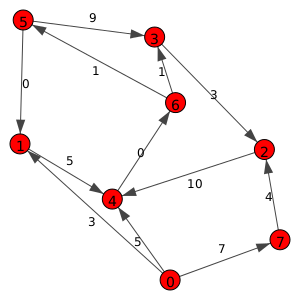
\includegraphics[width=\textwidth]{directgraph}
    \end{column}
    \begin{column}{0.58\textwidth}
      \begin{itemize}
      \item $G = (V,E)$ grafo
      \item $\abs{V} = N$, $\abs{E} = M$
      \item $V$ nodi
      \item $E \subseteq V\times V$ archi
      \item gli archi possono essere orientati
      \item gli archi possono avere un peso $w: E \to \mathbb{R}$ (nel
        nostro caso la lunghezza)
      \end{itemize}
    \end{column}
  \end{columns}
\end{frame}

\begin{frame}{Cammini}
  \begin{columns}
    \begin{column}{0.40\textwidth}
      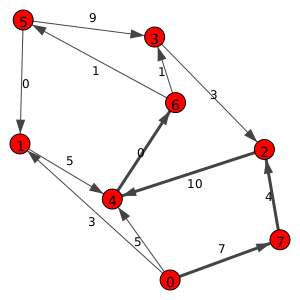
\includegraphics[width=\textwidth]{directpath}
    \end{column}
    \begin{column}{0.58\textwidth}
      \begin{itemize}
      \item Cammino: $p = \pa{ 0,7,2, 4,6}$
      \item Lunghezza: $w(p) = 7+4+10+0 = 21$
      \item $P(u,v) = \set{\text{cammini tra }u\text{ e }v}$
      \item Distanza: $\delta (u,v) = \min \limits _{p\in P(u,v)}
        w(p)$
      \item $\pa{V,\delta}$ \`e una pseudometrica
      \item I cammini minimi sono ``quasi'' aciclici
      \item Sottocammini di cammini minimi sono minimi
      \end{itemize}
    \end{column}
  \end{columns}
\end{frame}

\subsection{Cammini da una sorgente unica}

\begin{frame}{Grafo (aciclico diretto) dei cammini minimi}
  Scegliamo $s\in V$, vogliamo conoscere:
  \begin{itemize}
  \item $\forall v\in V\;\; \delta \pa{s,v}$
  \item $\forall v\in V$ i cammini minimi da $s$ a $v$
  \end{itemize}

  \begin{mypro}
    Se gli archi hanno lunghezza strettamente positiva, il grafo $G_s$
    dei cammini minimi \`e un DAG (grafo aciclico diretto)
  \end{mypro}
  Scegliendo opportunamente un cammino per ogni vertice otteniamo un
  albero.
\end{frame}

\begin{frame}{Archi non pesati: BFS}
    \begin{columns}
    \begin{column}{0.40\textwidth}
      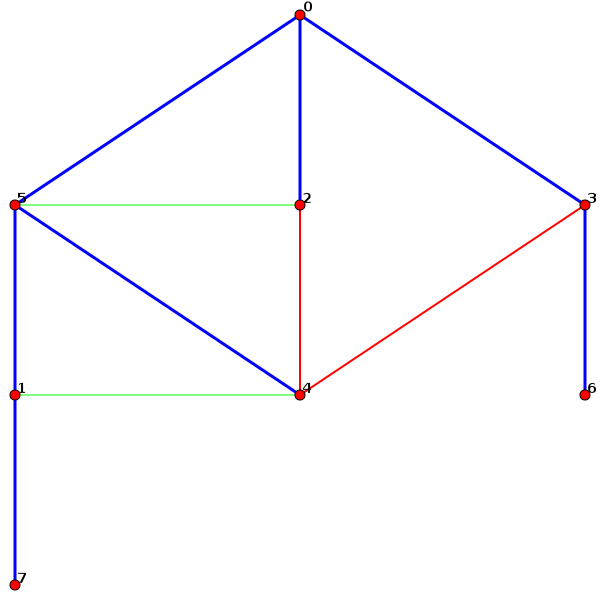
\includegraphics[width=\textwidth]{BFS}
    \end{column}
    \begin{column}{0.58\textwidth}
      Per grafi non pesati (archi di lunghezza unitaria) applicando
      una visita in ampiezza otteniamo distanze e cammini in
      $O\pa{M}$ operazioni.
    \end{column}
  \end{columns}
\end{frame}

\begin{frame}{Archi pesati: algoritmo di Dijkstra}
    \begin{columns}
    \begin{column}{0.40\textwidth}
      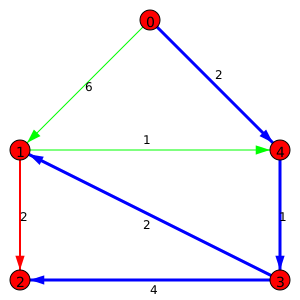
\includegraphics[width=\textwidth]{dijkstraslide} 
    \end{column}
    \begin{column}{0.58\textwidth}
      Per grafi pesati l'algoritmo di Dijkstra costruisce il DAG dei
      cammini minimi in $O\pa{M\log \pa{N}}$ operazioni.
    \end{column}
  \end{columns}  
\end{frame}

\subsection{Cammini tra tutte le coppie}

\begin{frame}{Matrice di adiacenza}
  Numeriamo i vertici: $V = \set{ 0,1,2,..., N-1}$.
  
  \vfill
  Definiamo la matrice $W$ dove
  \begin{itemize}
  \item $W_{i,i} = 0$
  \item $W_{i,j} = w(i,j)$ se $(i,j) \in E$
  \item $W_{i,j} = \infty$ se $(i,j) \not\in E$
  \end{itemize}
 
\end{frame}

\begin{frame}{Calcolo della matrice delle distanze}
  Matrice delle distanze: $d_{i,j} = \delta(i,j)$
  \vfill
  
  $l^{(m)}_{i,j} = \min\set{ l^{(m-1)} _{i,j} , \min _{0\le k\le N-1}
    \set{ l^{(m-1)} _{i,k} + w_{k,j}} }$
  
  Ogni cammino ha al pi\`u $N-1$ archi $\Rightarrow$ $d_{i,j} = l^{(N-1)}
  _{i,j}$.
  \vfill
  
  Possiamo riscrivere $l^{(m)}_{i,j} = \min \limits _{0\le k\le N-1}
  \set{ l^{(m-1)} _{i,k} + w_{k,j}}$
\end{frame}

\begin{frame}{Lettura del prodotto fra matrici}
  \begin{block}{}
    \begin{align*}
      l^{(m)}_{i,j} &=& & \min \limits _k & \Big\{ & l^{(m-1)}
      _{i,k} & & +  & & w_{k,j} \Big\} \\
      C_{i,j} &=& &\sum _k  & &  A_{i,k}  & & \cdot  & &B_{k,j} 
    \end{align*}
  \end{block}
  \pause
  
  \[ L^{(m)} = L^{(m-1)} * W \]

  \begin{block}{}
    \[ D = W^{N-1} \]
  \end{block}
\end{frame}

\begin{frame}{Complessit\`a}
  \begin{overprint}
    \onslide<1>
    \begin{center}
      \begin{tabular}{| c | c |}
        \hline
        Calcolo di un prodotto & Elevamento a potenza \\
        \hline
        $ A *B $ & $W ^N$ \\
        $O\pa{N^3}$ & $O\pa{ N}$ \\
        \hline
        \multicolumn{2}{| c| }{$O\pa{N^4}$}\\
        \hline
      \end{tabular}
    \end{center}
    \onslide<2>
    \begin{center}
      \begin{tabular}{| c | c |}
        \hline
        Calcolo di un prodotto & Elevamento a potenza \\
        \hline
        $ A *B $ & \cellcolor{yellow} $W ^{2^{\ceil{\log\pa{N}}}}$ \\
        $O\pa{N^3}$ & \cellcolor{yellow} $O\pa{ \log\pa{N}}$ \\
        \hline
        \multicolumn{2}{| c| }{$O\pa{N^3 \log\pa{N}}$}\\
        \hline
      \end{tabular}
    \end{center}
    \onslide<3->
    \begin{center}
      \begin{tabular}{| c | c |}
        \hline
        Calcolo di un prodotto & Elevamento a potenza \\
        \hline
        $ A *B $ & $W ^{2^{\ceil{\log\pa{N}}}}$ \\
        \color{red} \bf ??? $O\pa{N^\omega}$ ??? & $O\pa{ \log\pa{N}}$ \\
        \hline
        \multicolumn{2}{| c| }{\color{red} ?? $O\pa{N^\omega \log\pa{N}}$ ??}\\
        \hline
      \end{tabular}
    \end{center}
  \end{overprint}
  \vfill
  \begin{overprint}
    \onslide<3-> $O\pa{N^\omega}$ \`e la complessit\`a in tempo del
    prodotto veloce fra matrici.

    Il valore di $2\le\omega <3$ \`e un problema aperto.
  \end{overprint}
  \vfill
  \begin{overprint}
    \onslide<4-> Il prodotto veloce funziona solo su anelli.
    
    $\pa{\mathbb{R},\min, +}$ non \`e un anello!!
  \end{overprint}
  \vfill
  \begin{overprint}
    \onslide<5-> Per archi di peso intero positivo: $O\pa{ d N ^\omega
      \log d \log N}$
  \end{overprint}
\end{frame}


\begin{frame}{Altri risultati}
  \begin{itemize}
  \item Grafi senza cicli negativi: Floyd-Warshall $\rightarrow$ $O \pa{N^3}$
  \item Grafi con archi di peso intero positivo: SZ99 $\rightarrow$
    $\tilde O \pa{k N^\omega}$ (dove $k$ \`e la lunghezza massima di
    un arco).
  \end{itemize}
\end{frame}

\begin{frame}{Trovare i cammini minimi}
  \begin{mylem}
    Dati $u,v \in V$ e $u'$ vicino di $u$ si ha che esiste un cammino
    minimo in $P(u,v)$ che utilizza l'arco $(u,u')$ se e solo se
    \[ \delta \pa{ u,v} = w\pa{ u,u' } + \delta \pa{ u',v} \]
  \end{mylem}
  \vfill
  
  Questa relazione ci definisce i vicini di $u$ ``buoni'' per
  raggiungere $v$.
\end{frame}

\begin{frame}{Numero di cammini minimi}
  Dati due vertici il numero di cammini minimi tra i due potrebbe
  essere anche esponenziale
  \vfill
  
  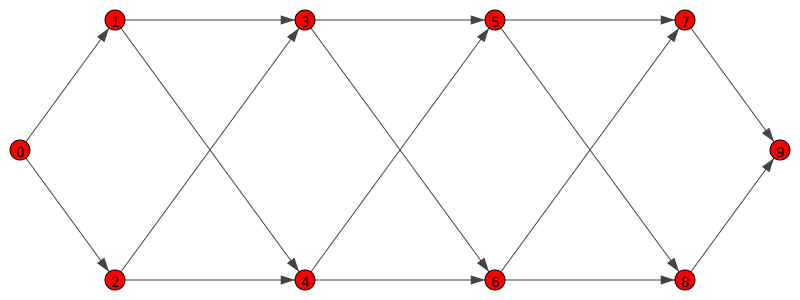
\includegraphics[width=\textwidth]{diamantecatena}
\end{frame}


\subsection{$k$ cammini pi\`u brevi}

\begin{frame}
  \begin{block}{Problema}
    Dati $u,v \in V$ trovare i $k$ cammini pi\`u brevi in $P(u,v)$.
  \end{block}
  \vfill
  
  \begin{itemize}
  \item Alcuni algoritmi venono forniti in Epp94
  \item In AL11, senza peggiorare le prestazioni al caso pessimo, si
    riesce a risolvere il problema senza esplorare tutto il grafo
  \end{itemize}
  
\end{frame}


\section{Oracoli per distanze}

\subsection{Oracoli approssimati}

\begin{frame}{Graph spanner}
  \begin{mydef}[$r$-approssimazione]
    Un algoritmo che ritorna $d(u,v)$ tale che
    \[ d\pa{u,v} \le r \delta\pa{u,v} \]
  \end{mydef}

  \begin{mydef}[$t$-spanner]
    $G' = (V,E')$ con $E' \subseteq E$ tale che la distanza in $G'$
    \`e una $t$-approssimazione.
  \end{mydef}

  \begin{myteo}
    Dato un grafo $G = (V,E)$ e due numeri $t,m\ge 1$ il problema di
    determinare se esiste un $t$-spanner di $G$ con al pi\`u $m$ archi
    \`e NP-completo.
  \end{myteo}
\end{frame}

\begin{frame}{Risultati}
  \begin{itemize}
  \item PS89: esiste un $(4r+1)$-spanner con $O(N^{1+1/r})$ vertici
  \item TODO
  \end{itemize}
\end{frame}

\subsection{Oracoli esatti}

\begin{frame}{Limiti teorici}
  \begin{itemize}
  \item Esistono $\binom{ N}{2}$ grafi con $N$ archi
  \item c'\`e una corrispondenza biunivoca tra grafi e tabelle delle
    distanze 
  \end{itemize}
  \pause
  \vfill
  Un oracolo deve saper distinugere tra $\binom{ N}{2}$ casi
  \pause
  \begin{block}{Lower bound}
    Un oracolo per distanze deve utilizzare almeno $N^2 / 2 + o(N^2)$
    bit
  \end{block}
\end{frame}

\begin{frame}{Albero etichettato}
  Sia $T$ un albero di ricoprimento qualsiasi di $T$ con radice in
  $r$. Denotiamo con $f(u)$ il padre di $u$.
  \vfill
  \[ \delta\pa{ s,u} = \delta\pa{ s,r} + \sum _{v\in \pi (u)} \bra{
    \delta\pa{ s,v} - \delta\pa{ s,f(v) } } \]
  
  Per la triangolare si ha $\abs{\delta\pa{ s,v} - \delta\pa{ s,f(v)}
  } \le \abs{\delta\pa{v,f(v)}} \le 1$ \vfill
  
  \pause
  \[ l_s(v) = \delta\pa{s,v} - \delta\pa{ s, f(v) } \in \set{
    -1,0,1} \]
\end{frame}

\begin{frame}{Somme prefisse}
  \begin{columns}
    \begin{column}{0.6\textwidth}
      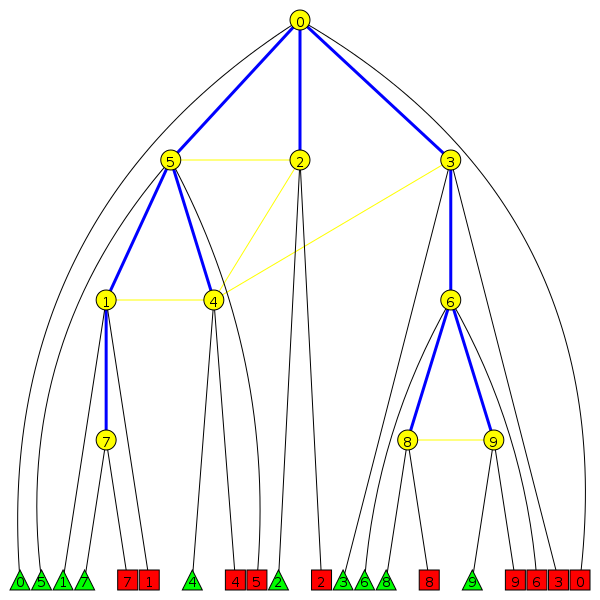
\includegraphics[width=\textwidth]{labeltree}
    \end{column}
    \begin{column}{0.39\textwidth}
      Associamo ad ogni etichettatura $l_s$ una sequenza $L_s$.

      Per ogni nodo $u\in V$ nella stringa compare $l(u)$ (triangolino
      verde) e $-l(u)$ (quadratino rosso).  \vfill \pause
      
      $\sum _{v\in \pi(u)} \bra{ \delta\pa{ s,v} - \delta\pa{ s,f(v) } }$
      \`e la somma prefissa fino a $r(u)$.
    \end{column}
  \end{columns}
\end{frame}

\begin{frame}{Complessità in spazio}
  Dobbiamo salvare:
  \begin{itemize}
  \item albero: $O\pa{N\log\pa{N}}$ bit
  \item distanze $\delta\pa{s,r}$ per ogni $s\in V$: $O\pa{ N \log N}$
    bit totali
  \item vettore $r$: $O\pa{N \log\pa{N}}$ bit 
  \item al variare di $s\in V$ il Wavelet Tree associato a $L_s$:
    $2\log\pa{3} N^2 + o(N^2)$ bit totali
  \end{itemize}
  \textbf{Totale:} ${2}\log\pa{3} N^2 + o(N^2)$ bit
  \vfill
  \pause

  Si pu\`o migliorare a 
  \begin{block}{Bit utilizzati}
    \[ \frac{1}{2}\log\pa{3} N^2 + o\pa{N^2} = 1.585 \frac{N^2}{2} +
    o\pa{N^2} \]
  \end{block}
\end{frame}


\section{Oracoli per cammini}

\subsection{Algoritmi facili}

\begin{frame}{Un oracolo}
  Supponiamo di conoscere la tabella delle distanze.
  \begin{mylem}
    Dati $u,v \in V$ e $u'$ vicino di $u$ esiste un cammino minimo in
    $P(u,v)$ che utilizza l'arco $(u,u')$ se e solo se $ \delta \pa{
      u,v} = w\pa{ u,u' } + \delta \pa{ u',v} $
  \end{mylem}
  \pause
  Per ogni $u,v\in V$ ci salviamo i vicini buoni di $u$ e procediamo
  in modo ricorsivo.
  \vfill \pause

  Spazio utilizzato: $O\pa{NM}$ bit.
\end{frame}

\begin{frame}{Un non oracolo}
  Invece di precalcolarci i vicini buoni, li troviamo durante
  l'elaborazione.
  
  Spazio utilizzato: un oracolo per distanze.
  \vfill
  \pause
  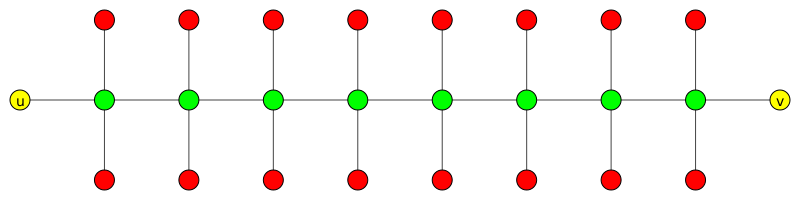
\includegraphics[width=\textwidth]{millepiedi}
  
  \begin{center}
    \textbf{Non \`e un oracolo!}
  \end{center}
\end{frame}

\subsection{Grafi planari}

\begin{frame}{Separation theorem}
  \begin{myteo}[\textit{Separation theorem}]
    Dato un grafo planare $G = (V,E)$ \`e possibile partizionare $V$
    in tre insiemi $A,B,S$ tali che
    \begin{itemize}
    \item $A$ e $B$ hanno al pi\`u $2N/3$ vertici ciascuno
    \item $S$ ha $O\pa{ \sqrt{N}}$ vertici
    \item non esistono archi tra $A$ e $B$
    \end{itemize}
  \end{myteo}
  \vfill
  \pause
  Sottografi di grafi planari sono planari, quindi possiamo applicare
  ricorsivamente il teorema a $A\cup S$ e $B\cup S$.
\end{frame}

\begin{frame}{Un oracolo}
  La struttura data dal \textit{separation theorem} ci permette di
  procedere con una strategia di \textit{divide et impera}.
  \vfill \pause

  Per ogni coppia $u,v\in V$ ci salviamo i nodi separanti ``buoni''
  che sono, al pi\`u, $O\pa{\sqrt{N}}$.
  \vfill \pause

  \begin{block}{Bit utilizzati}
    \[ O\pa{N^{2.5}} \]
  \end{block}
\end{frame}

\subsection{Miglioramenti dell'oracolo facile}

\begin{frame}{Miglioramento}
  
\end{frame}

\begin{frame}{Struttura dei cammini}
  
\end{frame}

\begin{frame}{Caso pessimo}
  
\end{frame}

\subsection{Costruzione di un caso difficile}

\begin{frame}{Grafo bipartito}
  
\end{frame}

\begin{frame}{Intersezione di insiemi}
  
\end{frame}


\end{document}







